\chapter{绪论}
\chaptermark{绪论}
	\section{研究背景}
	随着第二代高通量的测序技术的发展,测序通量在以超过摩尔定律增长趋势
		\subsection{基因组可视化}
		基因组可视化。
		\begin{figure}
			\centering
			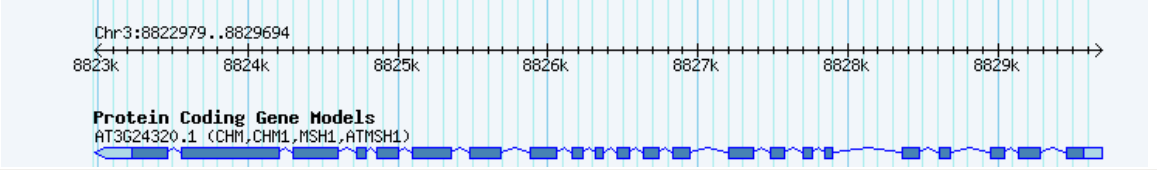
\includegraphics[width = .6\textwidth]{1-1.png}
			\caption{拟南芥可视化效果}
		\end{figure}
		该幅图片中包含了基因所在的染色体的信息(Chr3)、该基因在染色体上的坐标(8822979..8829694)、基因的名称和别名(AT3G24320.1、CHM等)、基因的方向(从右向左的箭头)、基因的组成单元(蓝色:外显子,曲线:内含子)。这些信息将成为基因组可视化中需要重点考虑的对象。
		\subsection{苹果基因组可视化}
		苹果作为悠久栽培历史的果树树种,在世界上产量排名第4,陕西省的苹果产量也位居全国第一位。
	\section{研究的目标和意义}
		\subsection{研究目标}
		本文以苹果基因组为数据源,以基因组可视化工具为主要研究对象,在可
		\subsection{研究意义}
		苹果作为悠久栽培历史的果树树种,在世界上产量排名第4。对于苹果基因
	\section{基因组可视化工具}
		\subsection{基因组可视化工具发展}
	基因组浏览器应该像人们平时使用高德地图、百度地图一样,实现某基因在
		\subsection{基于桌面和基于Web的基因组浏览器比较}
		根据基因组浏览器的使用形式,可以分为基于桌面的浏览器和web 浏览器
	\section{本文研究内容}
	本文的研究工作主要围绕苹果基因组的可视化问题展开, 
	\begin{enumerate}
		\item Linux环境选取及适配多种类型的Linux操作系统。 
		\item  Apache、MySQL的源码编译安装及配置,解决模块依赖问题。
		\item  GBrowse工具集安装及配置,解决与MySQL、Apache等关联问题。
		\item  JBrowse,UCSC Genome Browser的源码编译安装及配置,解决模块依赖问题。
		\item 苹果及其同源物种基因组数据集处理,及对相关数据及的整合调试。
		\item 对比不同web基因组浏览器的可视化效果,并对每种浏览器进行深入解析。
	\end{enumerate}
	
	\section{本文内容安排}
	本文第 1 章是绪论, 分为研究背景(对基因组及苹果基因组的可视化研究进展进行了简要介绍)、研究的目标和意义(主要说明了本文要达到的目标和